\subsection{Temperatur- og fugtsensor JS LB}


\begin{figure}[htb]
\centering
{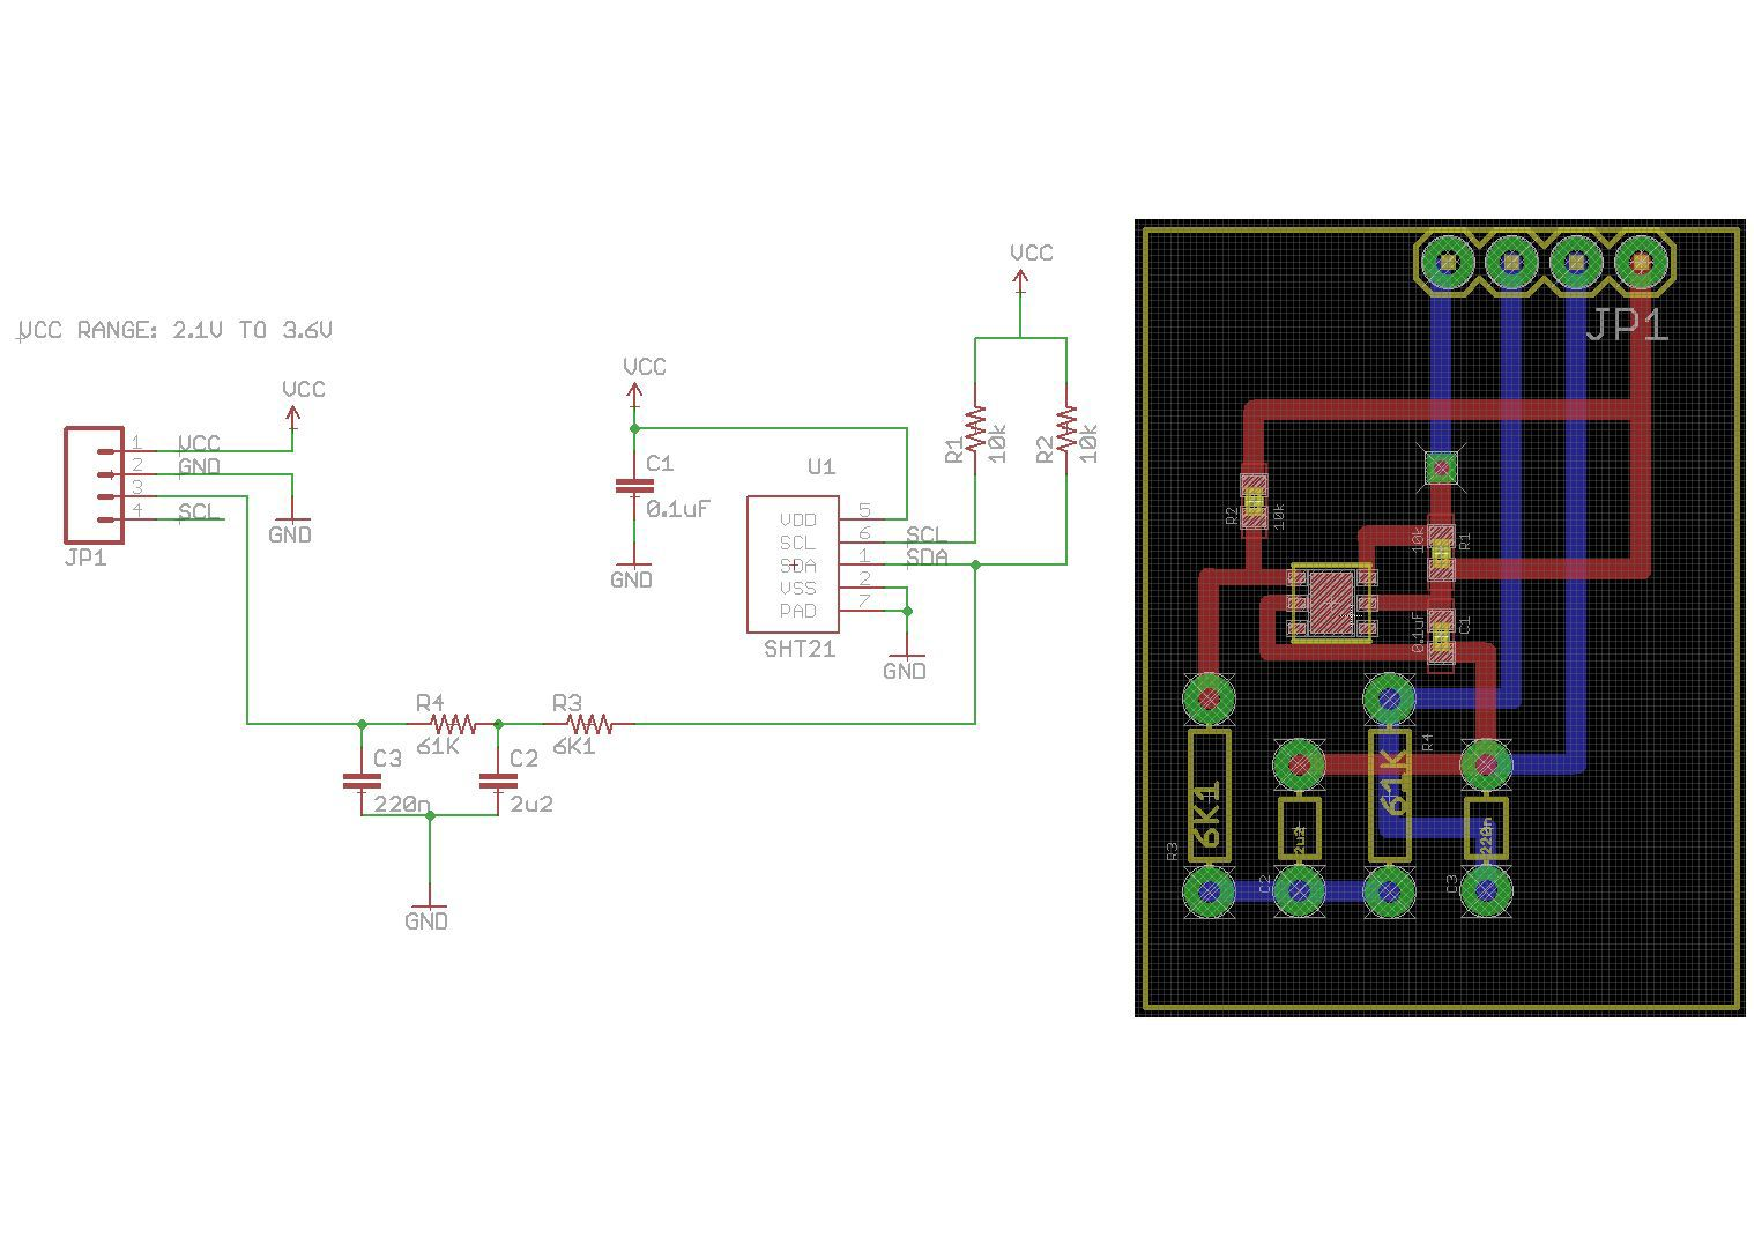
\includegraphics[width=\textwidth]{billeder/SHT_pcb}}
\caption{Schematic og layout af SHT21p kredsl\o{}b}
\label{lab:SHT21p-kredsloeb}
\end{figure}

Systemet indeholder  en fugt- og temperatur sensor. Sensorens opgave er at måle temperaturen og fugtigheden.
Sensoren udsender et PWM-signal, på ca. 120 Hz, hvor pulsbredden beskriver temperaturen og fugtigheden,  alt efter hvilken der er valgt. Det vælges med et høj eller lavt signal om der måles temperatur eller fugtighed, mere information om dette kan læses i dokumentation afsnit 5.2 Temperatur- og fugtsensor.
Da PSoC4s ADC-converter ikke kan læse et PWM-signal, skulle der findes en anden løsning. Løsningen blev at midle PWM-signalet så det bliver en DC-spænding som ADCen kan aflæse. Dette gøres med et 2. ordens lavpass-filter med en knækfrekvens på 12 Hz. Mere information om dette filter kan læses i afsnit 5.2.1 Midlingsfilter i dokumentationen. 
Der er også foretaget præcisions- og støjbehandling. Da nogen af komponenterne, som var til rådighed under projektet, havde en tolerance på $\pm$ 5\% har denne ikke været meget nødvendig. For yderligere information om præcisions- og støjbehandling, se dokumentationen afsnit 5.2.2 Præcisions- og støjhåndtering. 